\documentclass[letter]{article}

% Fields
\def\season{2024-2025}

\usepackage{titling}
\usepackage{graphicx}
\setlength{\columnseprule}{1pt}
\pretitle{%
  \AddToShipoutPictureBG*{%
  \begin{tikzpicture}[remember picture,overlay]
    \node[anchor=north west,scale=1.5] at (current page.north west){%
        \includegraphics{FIRSTLego_iconHorz_RGB}};
    \node[anchor=north east,scale=.11] at (current page.north east){%
        \includegraphics{FIRST_SUBMERGED_Patch_Logo_RGB}};
  \end{tikzpicture}}

  \begin{center}\Large\bfseries\MakeUppercase}
\author{}
      \title{First Lego League (FLL) \\ \season{} Season Charter}
\posttitle{%
\end{center}
\vspace{-2cm}
}
\date{}

\usepackage{geometry}
\geometry{margin=1in}
\usepackage{fancyhdr}

\usepackage[hidelinks]{hyperref}

\newcommand*{\SignatureAndDate}[1]{%
    \par\noindent\makebox[2.95in]{\hrulefill} \hfill\makebox[2.95in]{\hrulefill}%
    \par\noindent\makebox[2.95in][l]{Witness}      \hfill\makebox[2.95in][l]{#1}%
}%

\pagestyle{fancy}
\usepackage{lastpage}
\fancyhf{}
\fancyhead[L]{\season{} Season FLL Charter}
\fancyhead[R]{\thepage{} of \pageref{LastPage}}
\fancypagestyle{firststyle}
{
   \fancyhf{}
   \fancyfoot[C]{\footnotesize Page \thepage\ of \pageref{LastPage}}
   \renewcommand{\headrulewidth}{0pt} % removes horizontal header line
}

% Watermark
\usepackage{eso-pic}
\usepackage{tikz}
\AddToShipoutPictureFG{%
  \begin{tikzpicture}[remember picture,overlay]
    \node[gray,rotate=45,scale=14,opacity=0.2] at (current page.center){%
        \textbf{DRAFT}};
  \end{tikzpicture}}

% Calendar
\usetikzlibrary{calendar,shapes,positioning}
\makeatletter
\tikzstyle{week list sunday}=[
% Note that we cannot extend from week list,
% the execute before day scope is cumulative
execute before day scope={%
  \ifdate{day of month=1}{\ifdate{equals=\pgfcalendarbeginiso}{}{
      % On first of month, except when first date in calendar.
      \pgfmathsetlength{\pgf@y}{\tikz@lib@cal@month@yshift}%
      \pgftransformyshift{-\pgf@y}
    }}{}%
},
execute at begin day scope={%
  % Because for TikZ Monday is 0 and Sunday is 6,
  % we can't directly use \pgfcalendercurrentweekday,
  % but instead we define \c@pgf@counta (basically) as:
  % (\pgfcalendercurrentweekday + 1) % 7
  \pgfmathsetlength\pgf@x{\tikz@lib@cal@xshift}%
  \ifnum\pgfcalendarcurrentweekday=6
  \c@pgf@counta=0
  \else
  \c@pgf@counta=\pgfcalendarcurrentweekday
  \advance\c@pgf@counta by 1
  \fi
  \pgf@x=\c@pgf@counta\pgf@x
  % Shift to the right position for the day.
  \pgftransformxshift{\pgf@x}
},
execute after day scope={
  % Week is done, shift to the next line.
  \ifdate{Saturday}{
    \pgfmathsetlength{\pgf@y}{\tikz@lib@cal@yshift}%
    \pgftransformyshift{-\pgf@y}
  }{}%
},
% This should be defined, glancing from the source code.
tikz@lib@cal@width=7
]
\makeatother

\begin{document}
\maketitle
\thispagestyle{firststyle}

\hypertarget{communication}{%
\section{Communication}\label{communication}}

E-Mail distribution list. We compile an E-Mail distribution list from
recruitement events, parent requests and the orientation meeting. If you
would like to be added to the distribution list please email the head
coach at \href{mailto:ken@bellock.net}{\nolinkurl{ken@bellock.net}} and
request to be added to the list. If you are receiving emails and wish to
be removed from the list, reply (not reply-all) to an email with
``UNSUBSCRIBE'' in the subject line of the email.

\hypertarget{coach-profiles}{%
\section{Coach/Administrator Profiles}\label{coach-profiles}}

\hypertarget{omms-sponsor}{%
\subsection{OMMS Administrator}\label{omms-sponsor}}

This is a parent led club, but it would not be possible without
Mrs.~Hartman! She coordinates the creation of the teams, and provides us
with a space to practice, robots, legos, and game boards. Thank you
Mrs.~Hartman!!

\hypertarget{head-coach}{%
\subsection{Coach Bellock}\label{head-coach}}

My name is Ken Bellock, and I'll be the head coach for this season's FLL
teams. I have a B.S. in Mathematics and Physics from Penn State, and a
M.S. in Geographic Information Systems from Johns Hopkins. In the past I
worked for the space program as a contractor designing ascent aborts
scenarios for the Space Shuttle. For my current job I lead a team of
Embedded Software Engineers who automate tests on satellite systems
before we deploy them to space.

\hypertarget{coach-barcello}{%
\subsection{Coach Barcello}\label{coach-barcello}}

\hypertarget{coach-fletcher}{%
\subsection{Coach Fletcher}\label{coach-fletcher}}

I have a degree in Computer Science from Old Dominion University. I currently work for the Department of Defense and run a software and systems engineering group. I coached one of the two OMMS FLL teams in the 2023/2024 season.

\hypertarget{future-coaches}{%
\subsection{Future Coaches}\label{future-coaches}}

Coaching Help is Needed! We have several returning assistant coaches
this year, but we need more! If you are interested in helping out with
coaching please contact me and we can talk about how you can contribute.
Any and all help will be appreciated. You do not need to know anything about coding or building with legos to help out, and we are required to have at least two coaches per team we field during competition, and we could especially use assistance in the instruction of public speaking and pitch presentation.

\hypertarget{meeting-schedule}{%
\subsubsection{Meeting Schedule}\label{meeting-schedule}}

Thursdays 6-8pm except when the school is closed and on Halloween Usually
early after the new year we have competition (I do not know dates yet)
If we win a bracket, we move up and will have another day of
competition. Before competition we will meet on the weekends at a coach
or parents house to develop our robot game and presentation. These are
not required meetings, but are a lot of fun and very helpful for last
minute preparations for competion.

\begin{center}
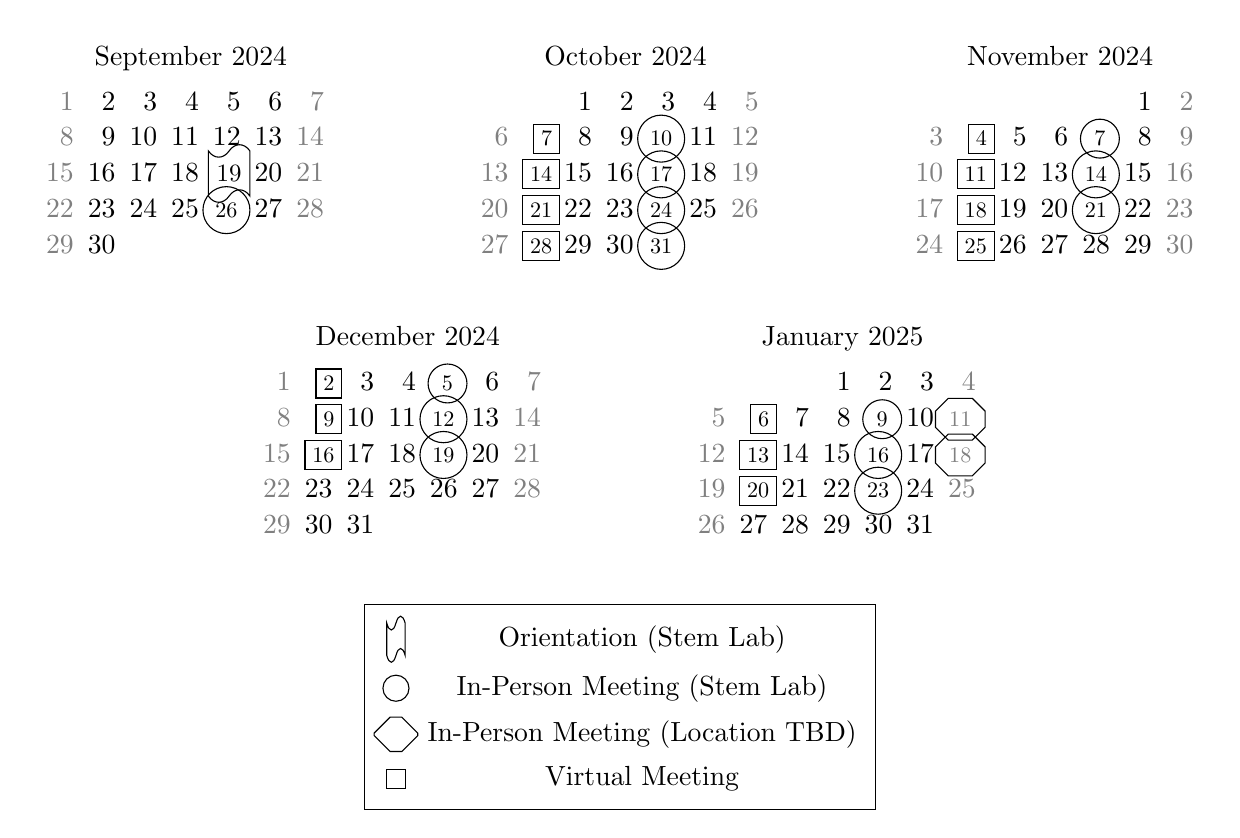
\begin{tikzpicture}[every calendar/.style = {
    month label above centered,
    month text = {\%mt \%y0},
    if={(weekend) [black!50]},
    week list sunday}]
  \matrix[column sep=5em, row sep=1em] {
    \calendar[dates=2024-09-01 to 2024-09-last]
      if (equals=2024-09-19) [nodes={tape,draw,scale=.9}]
      if (equals=2024-09-26) [nodes={circle,draw,scale=.8}]
    ; &
    \calendar[dates=2024-10-01 to 2024-10-last]
      if (equals=2024-10-07) [nodes={rectangle,draw,scale=.8}]
      if (equals=2024-10-10) [nodes={circle,draw,scale=.8}]
      if (equals=2024-10-14) [nodes={rectangle,draw,scale=.8}]
      if (equals=2024-10-17) [nodes={circle,draw,scale=.8}]
      if (equals=2024-10-21) [nodes={rectangle,draw,scale=.8}]
      if (equals=2024-10-24) [nodes={circle,draw,scale=.8}]
      if (equals=2024-10-28) [nodes={rectangle,draw,scale=.8}]
      if (equals=2024-10-31) [nodes={circle,draw,scale=.8}]
    ; &
    \calendar[dates=2024-11-01 to 2024-11-last]
      if (equals=2024-11-04) [nodes={rectangle,draw,scale=.8}]
      if (equals=2024-11-07) [nodes={circle,draw,scale=.8}]
      if (equals=2024-11-11) [nodes={rectangle,draw,scale=.8}]
      if (equals=2024-11-14) [nodes={circle,draw,scale=.8}]
      if (equals=2024-11-18) [nodes={rectangle,draw,scale=.8}]
      if (equals=2024-11-21) [nodes={circle,draw,scale=.8}]
      if (equals=2024-11-25) [nodes={rectangle,draw,scale=.8}]
    ; \\
  };
  \matrix[column sep=5em, row sep=1em,yshift=-10em] {
    \calendar[dates=2024-12-01 to 2024-12-last]
      if (equals=2024-12-02) [nodes={rectangle,draw,scale=.8}]
      if (equals=2024-12-05) [nodes={circle,draw,scale=.8}]
      if (equals=2024-12-09) [nodes={rectangle,draw,scale=.8}]
      if (equals=2024-12-12) [nodes={circle,draw,scale=.8}]
      if (equals=2024-12-16) [nodes={rectangle,draw,scale=.8}]
      if (equals=2024-12-19) [nodes={circle,draw,scale=.8}]
    ; &
    \calendar[dates=2025-01-01 to 2025-01-last]
      if (equals=2025-01-06) [nodes={rectangle,draw,scale=.8}]
      if (equals=2025-01-09) [nodes={circle,draw,scale=.8}]
      if (equals=2025-01-11) [nodes={chamfered rectangle,draw,scale=.8}]
      if (equals=2025-01-13) [nodes={rectangle,draw,scale=.8}]
      if (equals=2025-01-18) [nodes={chamfered rectangle,draw,scale=.8}]
      if (equals=2025-01-16) [nodes={circle,draw,scale=.8}]
      if (equals=2025-01-20) [nodes={rectangle,draw,scale=.8}]
      if (equals=2025-01-23) [nodes={circle,draw,scale=.8}]
    ; \\
  };
  \matrix[draw,yshift=-20em] {
      \node [tape,draw] {}; &
      \node {Orientation (Stem Lab)}; \\
      \node [circle,draw] {}; &
      \node {In-Person Meeting (Stem Lab)}; \\
      \node [chamfered rectangle,draw] {~~}; &
      \node {In-Person Meeting (Location TBD)}; \\
      \node [rectangle,draw] {}; &
      \node {Virtual Meeting}; \\
  };
\end{tikzpicture}
\end{center}

\hypertarget{game-overview}{%
\subsubsection{Game Overview}\label{game-overview}}

\href{https://youtu.be/c2f-Q5GGt2Q}{Season Promotional Video}

\href{https://youtu.be/J5u-2q_K3O0}{Robot Missions Overview}

Game Rules

Have Fun!

Students must do ALL of the work, coaches only provide guidance

Competition consists of the robot challenge, a core values presentation,
a conversation with judges about robot design, and an innovation project
presentation

Official Rulebook for Robot Competition:
\url{https://firstinspires.blob.core.windows.net/fll/challenge/2024-25/interactive-rgr/index.html}

Rubric for Presentations:
\url{https://firstinspires.blob.core.windows.net/fll/challenge/2024-25/fll-challenge-submerged-rubrics-color.pdf}

\hypertarget{interesting-notes}{%
\subsubsection{Interesting Notes}\label{interesting-notes}}

We are competing against over 35k teams through multiple brackets

We have never made it to the next level, but last year one of our teams
got real close, and every year we get better

\hypertarget{required-commitment}{%
\subsubsection{Required Commitment}\label{required-commitment}}

FLL is a team sport. Missing a meeting will hurt your team just like any
other team sport.

If you are not sure yet if you want to commit, please keep coming to the
next several meetings to help decide.

A commitment should be made by early October as that is when we will
create the teams that will work together until competition.

If you have days you know you will miss, please let us know as far in
advance as possible.

If too many days are missed, a critical role on competition day cannot
be guaranteed.

\hypertarget{behavioral-and-team-work-expectations-aka-gracious-professionalism}{%
\subsubsection{Behavioral and Team Work Expectations aka ``Gracious
Professionalism''}\label{behavioral-and-team-work-expectations-aka-gracious-professionalism}}

It's more than just good sportsmanship, it's treating our teammates and
opponents with respect, cooperation and professional behavior including
produtive communication skills. Words matter. Part of the robot
competition score is an evaluation of behavior. To practice on getting
the highest score for this part of the evaluation we are going to
practice ``Gracious Professionalism'' at all of our team meetings.

Finally, any major incidents that threaten the safety or well being of
any team member or coach may result in immediate suspension from the
club. Team members who display and escalate behaviors that involve name
calling, bad language, bullying, puposeful destruction of robots or
supplies, theft or physical altercations may be released immediatly from
FLL club participation.

\hypertarget{laptops}{%
\subsubsection{Laptops}\label{laptops}}

OMMS pays for registration, Legos, robots, and gives us space to
practice, but the laptops we are currently using have been donated. We
could use a few more laptops if anyone has old laptops that are not
being used. If you have laptops you do not use anymore, please consider
donating them to the team. They can be old, but must be working. Any
donated laptops will not be returned after the season ends. Students can
bring their own laptops, but we will not be responsible for lost, stolen
or broken laptops. I will send out instructions on how students can
contribute from home if they would like to. Any donated laptops will be
wiped clean and we will reinstall the operating system and the Lego
software

\hypertarget{phones}{%
\subsubsection{Phones}\label{phones}}

No phones are allowed out during meetings. You can bring them, but you
cannot have them out unless messaging a parent or guardian.

\hypertarget{what-else-to-bring-to-meetings}{%
\subsubsection{What Else To Bring To
Meetings}\label{what-else-to-bring-to-meetings}}

Send water bottles and snacks if you like

\hypertarget{fees}{%
\subsubsection{Fees}\label{fees}}

There are no registration or participation fees, but we will likely take
a collection as competition nears to get team shirts made. (If you can
make or design shirts and are willing, please let us know.) Thank you to
Jacen Scarberry's family who kindly helped us last year!

\hypertarget{final-notes}{%
\subsubsection{Final Notes}\label{final-notes}}

Legos, robots, missions and boards stay at school

If you have any questions please let me know. You can email me or we can
talk before or after meetings.



\end{document}

